\addbibresource{reference.bib}

\chapter{Energetická kalibrace}\label{calib}
Tato kapitola pojednává o metodách pro energetickou kalibraci hybridních částicových pixelových detektorů, pracujících v Time-Over-Treshold módu a o implementaci jedné z nich pro účely kalibrace detektorů sítě ATLAS TPX.

%********************************************************************************
% Motivace
%********************************************************************************
\section{Motivace}
Hybridní částicové pixelové detektory typu Timepix (viz \ref{det:tim}), disponují módem TOT (Time-Over-Treshold), který lze využít pro měření energie. Jak již bylo uvedeno v kapitole \ref{det:mod}, když částice interaguje s pixelem, pracujícím v tomto módu, ve kterém zanechá část své energie, dojde k vygenerování napěťového pulzu. Když je velikost tohoto pulzu větší, než treshold zasaženého pixelu, tak dojde je spuštění čítače, který začne počítat hodinové cykly měřící frekvence a zastaví se tehdy, když klesne hodnota napětí nazpět, pod úroveň tresholdu. Po skončení akvizice je hodnota tohoto čítače rovna hodnotě TOT, která zhruba odpovídá deponované energii interagující částice. Vztah mezi TOT a energií je ale silně nelineární a je podmíněn různými elektronickými a fyzikálními vlastnostmi daného pixelu. Určení tohoto vztahu je předmětem kalibrace, o které tato kapitola bude pojednávat.

%********************************************************************************
% Přehled kalibračních metod
%********************************************************************************
\section{Přehled kalibračních metod}

%********************************************************************************
% Přehled kalibračních metod
% > X-ray
%********************************************************************************
\subsection{Kalibrace detektorů za použití rentgenového záření}\label{calib:xray}
Metoda kalibrace pixelových detektorů pracujících v TOT módu \cite{Jakubek2011S262} spočívá v měření rentgenové fluorescence (viz \cite{Jakubek-radiography_and_charge_sharing}),
což je děj ke kterému dochází, když je nějaký materiál 
\footnote{Pro kalibraci se používají kovy, na příklad Am, In, Cu, Fe apod.}
ozařován rentgenovým zářením, které vyráží excitované elektrony z jeho atomů. Je-li vyražen elektron na nižší energetické úrovní, tak elektron z vyšší energetické úrovně deexcituje a obsadí jeho místo. Přebytečnou energii ztratí ve formě vyzářeného fotonu, který je následně detektorem detekován. 

Díky této fluorescenci je detektor pomocí různých mono-energetických zdrojů záření, jejichž energie je předem známa, postupně ozařován. V rámci tohoto měření je třeba pro každý zdroj pořídit velké množství snímků, ze kterých jsou následně vyfiltrovány jen tzv. \texttt{Single-Hit} události, což jsou události, při kterých interagující částice zasáhla jen jeden pixel. Tyto události jsou filtrovány z důvodu dosažení vyšší kvality kalibrace které je dosaženo potlačením zkreslení, způsobeným \texttt{Charge Sharing} efektem (viz \ref{det:mod}).

\begin{figure}[th]
	\begin{center}
		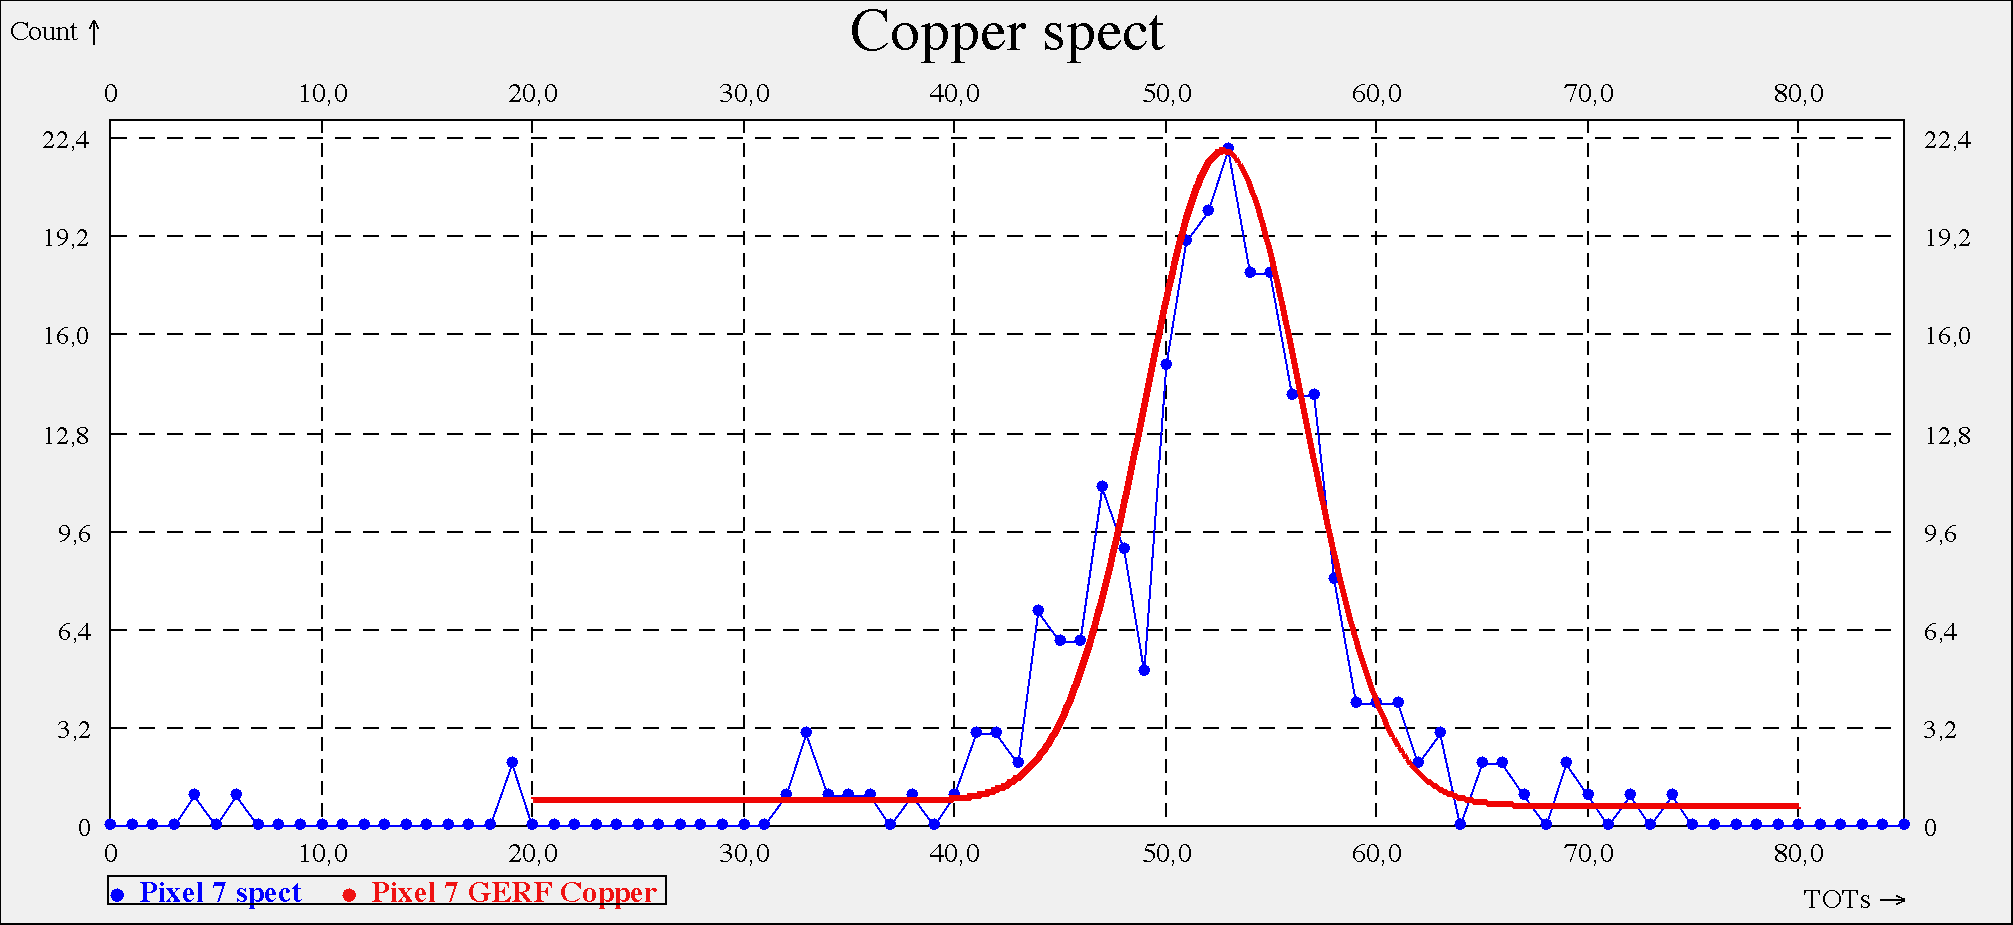
\includegraphics[width=14cm]{figures/calib_gerf.png}
		\caption{Spektrum TOT hodnot jednoho pixelu s proložením Gaussovou funkcí, sečtenou s Gaussovou chybovou funkcí (tzv. error funkce). Zdrojem rentgenové fluorescence byla měď.}
		\label{fig:calib:gerf}
	\end{center}
\end{figure}

Dalším krokem tohoto procesu je získání jednotlivých kalibračních bodů, udávající závislost mezi jednotlivými energiemi a TOT hodnotami. Toho je možné docílit vytvořením spekter pro jednotlivé pixely a zdroje záření. Na obrázku \ref{fig:calib:gerf} je příklad takového spektra pro jeden pixel detektoru a fluorescenčního záření z mědi. Na vodorovné ose tohoto spektra se nachází jednotlivé TOT hodnoty a na svislé pak jejich četnost ve všech snímcích. Z obrázku je patrné, že nejčetnější hodnotou TOT je zhruba hodnota $53$, které odpovídá energii fotonu, vyraženého z mědi, což je $5,9~keV$. Hodnotu TOT je ale třeba znát přesně, toho je docíleno proložením spektra funkcí \ref{eq:calib:gerf}, která vznikla z Gaussovy funkce, ke které z důvodu levé nesymetrie kvůli \texttt{Charge Sahring} efektu byla přičtena Gaussova chybová funkce. 

\begin{equation}\label{eq:calib:gerf}
	f_{GERF}(x) = \underbrace{Ae^{ -\frac{(x-\mu)^2}{2\sigma^2} }}_{\text{Gaussova funkce}} +
	\underbrace{ \frac{avg_{right} - avg_{left}}{\sigma\sqrt{2\pi}} \int_{-\infty}^t e^{ -\frac{(t-\mu)^2}{2\sigma^2} } + avg_{left}}_{\text{Gaussova chybová funkce}}
\end{equation}

Parametry funkce \ref{eq:calib:gerf} jsou následující:
\begin{itemize}
	\item $\mathbf{A}$ je amplituda.
	\item $\mathbf{\mu}$ je stření hodnota energie, kterou hledáme.
	\item $\mathbf{\sigma}$ udává rozptyl střední hodnoty energie a je možné ji vypočítat ze vzorce 
		$\sigma = \frac{2\sqrt{2ln_2}}{FWHM}$, kde $FWHM$\footnote{z angl. Full Width at Half Maximum} udává šířku gausiánu v polovině jeho výšky.
	\item $\mathbf{avg_{right}}$ (resp. $\mathbf{avg_{left}}$) je průměrná hodnoty spektra na pravém (resp. levém) úpatí gausiánu.
\end{itemize}
 
\begin{figure}[th]
	\begin{center}
		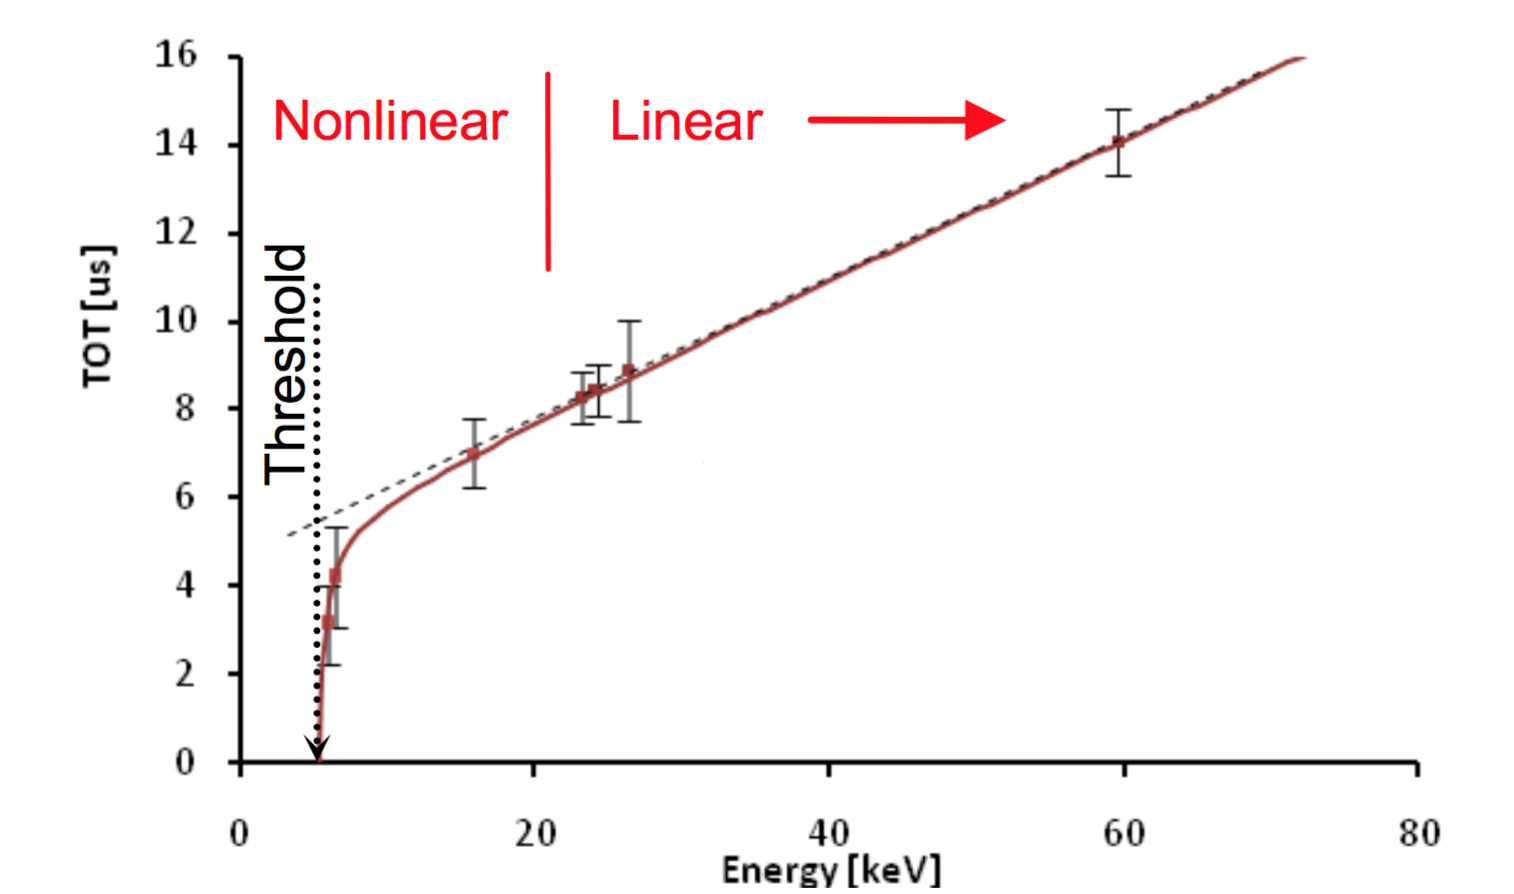
\includegraphics[width=13cm]{figures/calib_function.png}
		\caption{Kalibrační funkce (převzato z \cite{Jakubek2011S262})}
		\label{fig:calib:calib_function}
	\end{center}
\end{figure}

Z těchto kalibračních bodů je možné sestavit kalibrační funkci (viz vzorec \ref{eq:calib:calib_function}), udávající závislost mezi energií a TOT. Tato funkce vznikla složením hyperboly (popisující nelineární oblast nižších energií) a přímky (pro oblast s vyšší energií). Na obrázku \ref{fig:calib:calib_function} je znázorněn příklad této funkce.

\begin{equation}\label{eq:calib:calib_function}
	f_{calib}(x) = ax + b - \frac{c}{x-t}
\end{equation}


%********************************************************************************
% Přehled kalibračních metod
% > LED
%********************************************************************************
\subsection{Kalibrace detektorů pomocí LED diod}
Princip kalibrace pixelových detektorů (pracujících v TOT módu) pomocí LED diod spočívá v působení přesného množství světelného záření na polovodičový senzor detektoru. V současné době je tato metoda ve fázi vývoje a doposud nebyla publikována. Metoda je použitelná pouze pro detektory, na jejímž senzoru není napařena tenká vrstva hliníku, která světelné záření nepropouští. 

Jako zdroj světla byl v ÚTEF ČVUT v Praze vyvinut modul s maticí $8\times8$ LED diod, který je možné ovládat pomocí \texttt{RS232} sériové linky. K tomuto modulu byl rovněž vyvinut plugin do softwarového balíku Pixelman \ref{det:pixelman}, který automatizuje proces nabírání dat této metody. Přes sériovou linku je schopen řídit modul s LED diodami a zároveň pomocí jádra Pixelmanu ovládá akvizici dat detektoru.

Kroky algoritmu této kalibrace jsou následující:
\begin{enumerate}
	\item Inicializace - nastavení spouštění akvizice detektoru na externí hardwarový trigger (který bude ovládán modulem s LED diodami), nastavení energie světelného záření (počet zabliknutí diody, délka periody jednoho bliknutí a doba aktivace diody v jedné periodě) a také délku akvizice snímku (vypočtené dle periody blikání a počet opakování).
	\item Měřící smyčka (opakuje se pro všechny LED diody). V rámci jednoho průchodu se provede následující:
		\begin{itemize}
			\item Zamaskování všech pixelů detektoru, krom těch pixelů, které jsou pod aktivní diodou.
			\item Spuštění akvizice.
			\item Vyčtení a uložení snímku z detektoru.
		\end{itemize}
	\item Následně se hodnoty všech snímků sečtou do jednoho snímku - viz obr. \ref{fig:calib:led_frame}.
\end{enumerate}

\begin{figure}[th]
	\begin{center}
		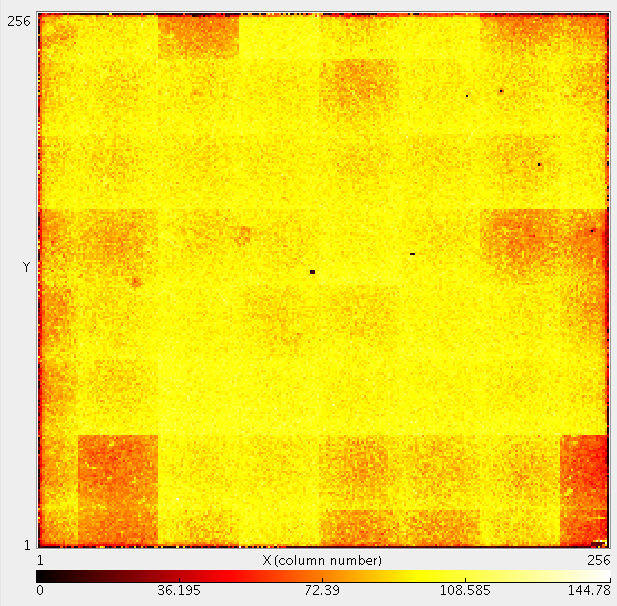
\includegraphics[width=10cm]{figures/led_calib_frame.png}
		\caption{Snímek z detektoru, ozařovaném modulem s LED diodami}
		\label{fig:calib:led_frame}
	\end{center}
\end{figure}

Z obrázku \ref{fig:calib:led_frame} jsou patrné hrany jednotlivých dílčích měření, které vznikly nehomogenitou elektronických vlastností jednotlivých diod. Tento jev může být odstraněn normalizací jejich světelné intenzity jejich kalibrací, jejíž výstupem bude kalibrační matice, kterou se vynásobí čas aktivace každé diody, což bude předmětem dalšího výzkumu této metody.

Tímto způsobem se pro každý pixel detektoru získají jednotlivé kalibrační body, které se následně proloží kalibrační funkcí (viz vzorec \ref{eq:calib:calib_function}), jak již bylo popsáno v kapitole \ref{calib:xray}.


%********************************************************************************
% X-ray Calib impl
%********************************************************************************
\section{Software pro kalibraci detektorů za použití rentgenového záření}

% osnova:
% výběr vstupních dat
% analýza spekter
% vytvoření kalibrační funkce (+ uložení dat apod.)
% výs































